% $Header: /cvsroot/latex-beamer/latex-beamer/examples/beamerexample5.tex,v 1.22 2004/10/08 14:02:33 tantau Exp $

\documentclass[10pt,xcolor=dvipsnames]{beamer}

\usetheme{JuanLesPins}

\usepackage{listings}
\usepackage{times}
\usepackage{amsmath}
\usepackage{amssymb}
\usepackage{epsfig}
\usefonttheme{structurebold}

\usepackage[english]{babel}
\usepackage{pgf,pgfarrows,pgfnodes,pgfautomata,pgfheaps}
\usepackage{amsmath,amssymb}
\usepackage[latin1]{inputenc}
%\usepackage{moreverb}

\setbeamercovered{dynamic}

\newcommand{\Lang}[1]{\operatorname{\text{\textsc{#1}}}}

\newcommand{\Class}[1]{\operatorname{\mathchoice
  {\text{\sf \small #1}}
  {\text{\sf \small #1}}
  {\text{\sf #1}}
  {\text{\sf #1}}}}

\newcommand{\NumSAT}      {\text{\small\#SAT}}
\newcommand{\NumA}        {\#_{\!A}}

\newcommand{\barA}        {\,\bar{\!A}}

\newcommand{\pd}[2]{\frac{\partial #1}{\partial #2}}
\newcommand{\od}[2]{\frac{d #1}{d #2}}
\newcommand{\pdd}[2]{\frac{\partial^2 #1}{\partial #2^2}}
\newcommand{\pddd}[2]{\frac{\partial^3 #1}{\partial #2^3}}
\newcommand{\pmix}[3]{\frac{\partial^2 #1}{\partial #2 \partial #3}}
\newcommand{\pmixx}[4]{\frac{\partial^3 #1}{\partial #2 \partial #3 \partial #4}}
\newcommand{\evalat}[2]{\left.#1\right\vert_{#2}}
\newcommand{\parent}{\mathrm{parent}}

\newcommand{\Nat}{\mathbb{N}}
\newcommand{\Set}[1]{\{#1\}}
\newcommand{\op}[1]{{\mathcal{#1}}}

\pgfdeclaremask{tu}{beamer-tu-logo-mask}
\pgfdeclaremask{computer}{beamer-computer-mask}
\pgfdeclareimage[interpolate=true,mask=computer,height=2cm]{computerimage}{beamer-computer}
\pgfdeclareimage[interpolate=true,mask=computer,height=2cm]{computerworkingimage}{beamer-computerred}
\pgfdeclareimage[mask=tu,height=.5cm]{logo}{beamer-tu-logo}

\logo{\pgfuseimage{logo}}


\title{Automated Self-Assembly of Components for Multiphysics Simulations}
\author{K. Long}
\institute[TTU]{%
Department of Mathematics and Statistics\\
Texas Tech University}
\date{SIAM Conference on Parallel Computing \\ 26 Feb 2010 }

\colorlet{redshaded}{red!25!bg}
\colorlet{shaded}{black!25!bg}
\colorlet{shadedshaded}{black!10!bg}
\colorlet{blackshaded}{black!40!bg}

\colorlet{darkred}{red!80!black}
\colorlet{darkblue}{blue!80!black}
\colorlet{darkgreen}{green!80!black}


\def\radius{0.96cm}
\def\innerradius{0.85cm}

\def\softness{0.4}
\definecolor{softred}{rgb}{1,\softness,\softness}
\definecolor{softgreen}{rgb}{\softness,1,\softness}
\definecolor{softblue}{rgb}{\softness,\softness,1}

\definecolor{softrg}{rgb}{1,1,\softness}
\definecolor{softrb}{rgb}{1,\softness,1}
\definecolor{softgb}{rgb}{\softness,1,1}

\newcommand{\Bandshaded}[2]{
  \color{shadedshaded}
  \pgfmoveto{\pgfxy(-0.5,0)}
  \pgflineto{\pgfxy(-0.6,0.1)}
  \pgflineto{\pgfxy(-0.4,0.2)}
  \pgflineto{\pgfxy(-0.6,0.3)}
  \pgflineto{\pgfxy(-0.4,0.4)}
  \pgflineto{\pgfxy(-0.5,0.5)}
  \pgflineto{\pgfxy(4,0.5)}
  \pgflineto{\pgfxy(4.1,0.4)}
  \pgflineto{\pgfxy(3.9,0.3)}
  \pgflineto{\pgfxy(4.1,0.2)}
  \pgflineto{\pgfxy(3.9,0.1)}
  \pgflineto{\pgfxy(4,0)}
  \pgfclosepath
  \pgffill

  \color{black}
  \pgfputat{\pgfxy(0,0.7)}{\pgfbox[left,base]{#1}}
  \pgfputat{\pgfxy(0,-0.1)}{\pgfbox[left,top]{#2}}
}

\newcommand{\Band}[2]{
  \color{shaded}
  \pgfmoveto{\pgfxy(-0.5,0)}
  \pgflineto{\pgfxy(-0.6,0.1)}
  \pgflineto{\pgfxy(-0.4,0.2)}
  \pgflineto{\pgfxy(-0.6,0.3)}
  \pgflineto{\pgfxy(-0.4,0.4)}
  \pgflineto{\pgfxy(-0.5,0.5)}
  \pgflineto{\pgfxy(4,0.5)}
  \pgflineto{\pgfxy(4.1,0.4)}
  \pgflineto{\pgfxy(3.9,0.3)}
  \pgflineto{\pgfxy(4.1,0.2)}
  \pgflineto{\pgfxy(3.9,0.1)}
  \pgflineto{\pgfxy(4,0)}
  \pgfclosepath
  \pgffill

  \color{black}
  \pgfputat{\pgfxy(0,0.7)}{\pgfbox[left,base]{#1}}
  \pgfputat{\pgfxy(0,-0.1)}{\pgfbox[left,top]{#2}}
}

\newcommand{\BaenderNormal}
{%
  \pgfsetlinewidth{0.4pt}
  \color{black}
  \pgfputat{\pgfxy(0,5)}{\Band{input tapes}{}}
  \pgfputat{\pgfxy(0.35,4.6)}{\pgfbox[center,base]{$\vdots$}}
  \pgfputat{\pgfxy(0,4)}{\Band{}{}}

  \pgfxyline(0,5)(0,5.5)
  \pgfxyline(1.2,5)(1.2,5.5)
  \pgfputat{\pgfxy(0.25,5.25)}{\pgfbox[left,center]{$w_1$}}

  \pgfxyline(0,4)(0,4.5)
  \pgfxyline(1.8,4)(1.8,4.5)
  \pgfputat{\pgfxy(0.25,4.25)}{\pgfbox[left,center]{$w_n$}}
  \ignorespaces}

\newcommand{\BaenderZweiNormal}
{%
  \pgfsetlinewidth{0.4pt}
  \color{black}
  \pgfputat{\pgfxy(0,5)}{\Band{Zwei Eingabeb�nder}{}}
  \pgfputat{\pgfxy(0,4.25)}{\Band{}{}}

  \pgfxyline(0,5)(0,5.5)
  \pgfxyline(1.2,5)(1.2,5.5)
  \pgfputat{\pgfxy(0.25,5.25)}{\pgfbox[left,center]{$u$}}

  \pgfxyline(0,4.25)(0,4.75)
  \pgfxyline(1.8,4.25)(1.8,4.75)
  \pgfputat{\pgfxy(0.25,4.5)}{\pgfbox[left,center]{$v$}}
  \ignorespaces}

\newcommand{\BaenderHell}
{%
  \pgfsetlinewidth{0.4pt}
  \color{black}
  \pgfputat{\pgfxy(0,5)}{\Bandshaded{input tapes}{}}
  \color{shaded}
  \pgfputat{\pgfxy(0.35,4.6)}{\pgfbox[center,base]{$\vdots$}}
  \pgfputat{\pgfxy(0,4)}{\Bandshaded{}{}}

  \color{blackshaded}
  \pgfxyline(0,5)(0,5.5)
  \pgfxyline(1.2,5)(1.2,5.5)
  \pgfputat{\pgfxy(0.25,5.25)}{\pgfbox[left,center]{$w_1$}}

  \pgfxyline(0,4)(0,4.5)
  \pgfxyline(1.8,4)(1.8,4.5)
  \pgfputat{\pgfxy(0.25,4.25)}{\pgfbox[left,center]{$w_n$}}
  \ignorespaces}

\newcommand{\BaenderZweiHell}
{%
  \pgfsetlinewidth{0.4pt}
  \color{black}
  \pgfputat{\pgfxy(0,5)}{\Bandshaded{Zwei Eingabeb�nder}{}}%
  \color{blackshaded}
  \pgfputat{\pgfxy(0,4.25)}{\Bandshaded{}{}}
  \pgfputat{\pgfxy(0.25,4.5)}{\pgfbox[left,center]{$v$}}
  \pgfputat{\pgfxy(0.25,5.25)}{\pgfbox[left,center]{$u$}}%

  \pgfxyline(0,5)(0,5.5)
  \pgfxyline(1.2,5)(1.2,5.5)

  \pgfxyline(0,4.25)(0,4.75)
  \pgfxyline(1.8,4.25)(1.8,4.75)
  \ignorespaces}

\newcommand{\Slot}[1]{%
  \begin{pgftranslate}{\pgfpoint{#1}{0pt}}%
    \pgfsetlinewidth{0.6pt}%
    \color{structure}%
    \pgfmoveto{\pgfxy(-0.1,5.5)}%
    \pgfbezier{\pgfxy(-0.1,5.55)}{\pgfxy(-0.05,5.6)}{\pgfxy(0,5.6)}%
    \pgfbezier{\pgfxy(0.05,5.6)}{\pgfxy(0.1,5.55)}{\pgfxy(0.1,5.5)}%
    \pgflineto{\pgfxy(0.1,4.0)}%
    \pgfbezier{\pgfxy(0.1,3.95)}{\pgfxy(0.05,3.9)}{\pgfxy(0,3.9)}%
    \pgfbezier{\pgfxy(-0.05,3.9)}{\pgfxy(-0.1,3.95)}{\pgfxy(-0.1,4.0)}%
    \pgfclosepath%
    \pgfstroke%
  \end{pgftranslate}\ignorespaces}

\newcommand{\SlotZwei}[1]{%
  \begin{pgftranslate}{\pgfpoint{#1}{0pt}}%
    \pgfsetlinewidth{0.6pt}%
    \color{structure}%
    \pgfmoveto{\pgfxy(-0.1,5.5)}%
    \pgfbezier{\pgfxy(-0.1,5.55)}{\pgfxy(-0.05,5.6)}{\pgfxy(0,5.6)}%
    \pgfbezier{\pgfxy(0.05,5.6)}{\pgfxy(0.1,5.55)}{\pgfxy(0.1,5.5)}%
    \pgflineto{\pgfxy(0.1,4.25)}%
    \pgfbezier{\pgfxy(0.1,4.25)}{\pgfxy(0.05,4.15)}{\pgfxy(0,4.15)}%
    \pgfbezier{\pgfxy(-0.05,4.15)}{\pgfxy(-0.1,4.2)}{\pgfxy(-0.1,4.25)}%
    \pgfclosepath%
    \pgfstroke%
  \end{pgftranslate}\ignorespaces}

\newcommand{\ClipSlot}[1]{%
  \pgfrect[clip]{\pgfrelative{\pgfxy(-0.1,0)}{\pgfpoint{#1}{4cm}}}{\pgfxy(0.2,1.5)}\ignorespaces}

\newcommand{\ClipSlotZwei}[1]{%
  \pgfrect[clip]{\pgfrelative{\pgfxy(-0.1,0)}{\pgfpoint{#1}{4.25cm}}}{\pgfxy(0.2,1.25)}\ignorespaces}


\AtBeginSection[]{\frame{\frametitle{Outline}\tableofcontents[current]}}

\begin{document}

\frame{\titlepage}




%\section*{Outline}
\part{Main Part}
\frame{\frametitle{Outline}\tableofcontents[part=1]}

\section{High-level problem specifications}

\begin{frame}[fragile]

\frametitle{High-level specification of a PDE}

  \lstset{language=C++,tabsize=2,basicstyle=\scriptsize}
  \begin{block}{Fragment of user-level code for Poisson equation}
  \begin{lstlisting}
   /* Create unknown and test functions, discretized using first-order
    * Lagrange interpolants */
   Expr u = new UnknownFunction(new Lagrange(2), "u");
   Expr v = new TestFunction(new Lagrange(2), "v");

   /* Create differential operator and coordinate function */
   Expr dx = new Derivative(0);
   Expr x = new CoordExpr(0);

   /* Define the weak form */
   Expr eqn = Integral(interior, -(dx*v)*(dx*u), quad)
        + Integral(interior, -2.0*v, quad);
   /* Define the Dirichlet BC */
   Expr bc = EssentialBC(leftPoint, v*u, quad);

   /* Put together a linear problem */
   LinearProblem prob(mesh, eqn, bc, v, u, vecType);
  \end{lstlisting}
  \end{block}

\end{frame}


\frame
{
  \frametitle{Goals and approach}
  \begin{block}{From high level to low level}
  \begin{itemize}
  \item High-level description encodes specification of low-level tasks
  \item The key to retaining performance is to distinguish high-level specification objects from
low-level computational kernels
  \item High-level description encodes structural information we
can exploit to improve performance
\begin{itemize}
\item For example, identify and eliminate redundant computations
\end{itemize}
  \item Optimization of computational kernels then apply to any
simulation built from them
  \item Our job is to ``build the matrix'' (or effect an MV multiply)
  \end{itemize}
  \end{block}

}

\frame
{
  \frametitle{The Sundance toolkit}
  \begin{block}{Ideas implemented in Sundance toolkit}
  \begin{itemize}
  \item Sundance is a Trilinos package
  \item Available from {\tt trilinos.sandia.gov}
  \end{itemize}
  \end{block}

}


\section{Automating simulation self-assembly from high-level interfaces}


\subsection{Mathematical foundations}


\frame
{
  \frametitle{Preliminaries}

  \begin{block}{Functionals}
  We work with functionals $F : (V,U) \rightarrow \mathbb{R}$ of the form
\[
  F\left[v,u,\right] = \int_{\Omega} \mathcal{F}(v,u) \, dx
\]
 where $\mathcal{F}$
\begin{itemize}
\item can be a {\bf nonlinear} differential operator
on $u$
\item but must be a {\bf linear, homogeneous} differential operator on $v$.
\end{itemize}
  \end{block}
\begin{block}{Weak Equations}
  We are interested in equations of the form
\[
  F\left[v,u\right] = 0 \;\;\; \forall v \in V
\]
  \end{block}
}


\frame
{
  \frametitle{Expository simplifications}

  \begin{block}{To keep notation compact during talk:}
  \begin{itemize}
  \item Assume the same equations apply over whole domain
  \begin{itemize}
  \item Trivially extended to multiple domains
  \end{itemize}
  \item Ignore boundary conditions
  \begin{itemize}
  \item Many BC methods (e.g., Nitsche) fit immediately into the framework
as shown
  \item Replacement BC methods require some annotation at user
level and conditionals in matrix assembly, but otherwise fit into our
framework
  \end{itemize}
  \end{itemize}
  \end{block}
}

\frame
{
  \frametitle{Examples of some functionals}

  \begin{block}{Steady Navier-Stokes flow}
\[
  F\left[\mathbf{v},\mathbf{u},q,p\right] = \int_\Omega
\left[\nu \nabla\mathbf{v} :\nabla\mathbf{u} + p \nabla \cdot\mathbf{v}
+ \mathbf{v}\cdot\left(\mathbf{u}\cdot\nabla\right)\mathbf{u}
+ q \nabla\cdot\mathbf{u}\right]
\]
  \end{block}

  \begin{block}{Lagrangian for Poisson source inversion w/ Tikhonov}
\begin{multline*}
  F\left[v,\mu,\beta,u,\lambda,\alpha\right]
= \int_\Omega \left[\left(u-u^*\right) v +  \nabla\lambda\cdot\nabla v \right]\, dx
+ \\
+ \int_\Omega \left[\nabla\mu\cdot\nabla u + \mu\alpha\right] \, dx + \\
+ \int_\Omega \left[\nabla \alpha \cdot \nabla\beta + \lambda \beta\right]\, dx
\end{multline*}
  \end{block}
}


\frame
{
  \frametitle{Discretization}

\begin{block}{}
\begin{itemize}
\item Introduce $N$-dimensional subspaces $V^h$ and $U^h$, with bases
$\left\{\psi_i\right\}_{i=1}^N$ and $\left\{\phi_i\right\}_{i=1}^N$.
\item Introduce $v^h = \sum_{i=1}^N \mathbf{v}_i\psi_i$
and $u^h = \sum_{i=1}^N \mathbf{u}_i\phi_i$
where $\mathbf{v}$ and $\mathbf{u}$ are vectors of expansion coefficients.
\end{itemize}
\end{block}
\begin{block}{}
\begin{itemize}
\item Approximation on spaces $V^h,U^h$ takes $F\left[v,u\right]$
to
\[
{\hat F}(\mathbf{v},\mathbf{u}) : (\mathbb{R}^N, \mathbb{R}^N) \rightarrow \mathbb{R}.
\]
\item The equation $F\left[v,u\right]=0 \; \forall\, v \in V$ becomes
\[{\hat F}(\mathbf{v},\mathbf{u})=0 \; \forall\, \mathbf{v}\in\mathbb{R}^N.\]
\end{itemize}
\end{block}
}

\frame
{
  \frametitle{A simple but consequential lemma}

\begin{lemma}
${\bf u}^*$ is a solution of
${\hat F}(\mathbf{v},\mathbf{u})=0 \;\;\; \forall\, \mathbf{v}\in\mathbb{R}^N$
iff
\[
\evalat{\pd{\hat F}{v_i}}{\mathbf{v}=0,\mathbf{u}=\mathbf{u}^*}=0,
\;\;\;i=1:N 
\]
\end{lemma}
\only<1>
{
  \begin{proof}
  Follows immediately from linearity \& homogeneity of $F$ as it acts on $\mathbf{v}$.
  \end{proof}
}
\only<2>
{
  \begin{block}{Derivatives are with respect to {\it test functions}}
  Not to be confused with first-order optimality conditions for a variational problem
  \end{block}
}
}

\frame
{
\frametitle{Differentiation provides the path to automation}
\begin{block}{A simple theorem establishes these relations}
\[
\pd{F}{v_i} =
\sum_\alpha \int_\Omega \pd{\mathcal{F}}{D_\alpha v} D_\alpha \psi_i
\]
\[
\pmix{F}{v_i}{u_j}
= \sum_{\alpha,\beta} \int_\Omega \pmix{\mathcal{F}}{D_\alpha v}{D_\beta u}
\, D_\alpha \psi_i \, D_\beta \phi_j
\]
\end{block}
\begin{alertblock}{\begin{center}The key idea\end{center}}
This theorem bridges high-level problem specification and low-level computation!
Fr\'echet differentiation connects:
\begin{itemize}
{\footnotesize
\item The abstract problem specification $\mathcal{F}$
\item The discretization specification: $\psi$, $\phi$, and integration procedure
\item The discrete matrix and vector elements $\pmix{F}{v_i}{u_j}$ and $\pd{F}{v_i}$
}
\end{itemize}
\end{alertblock}
}


\subsection{Software architecture}

\frame
{
  \frametitle{A plan for automation}

\begin{block}{To make practical use of the bridge theorem we need:}
\begin{itemize}
\item A data structure for high-level symbolic description of functionals $F$
\item Integrands $\mathcal{F}$ represented as DAG
\item Automated selection of basis function combinations from element library,
given signature of derivative
\item Connection to finite element infrastructure for basis functions, mesh, quadrature,
linear algebra, and solvers
\item A top-level layer for problem specification
\item A method to automate the organization of efficient
in-place computations of {\it numerical values} of $\pd{\mathcal{F}}{v}$, etc, given DAG for $\mathcal{F}$
\item Low-level AD tools not suitable
\end{itemize}
\end{block}
}


\frame
{
\frametitle{Example: Burgers' Equation}

\begin{block}{Weak form of Burgers' equation on $\left[0,1\right]$}
\[
\int_0^1 \left[v u D_x u + c D_x v D_x u \right] \, dx = 0
\;\;\;\;\forall v\in H^1_\Omega.
\]
(Ignoring BCs)
\end{block}
}

\frame
{
\frametitle{Burgers' Example: Mapping from Derivative Signature
to Coefficient and Basis Combination}
\begin{block}{}
{\footnotesize
\[
\begin{array}{|c|c|c|c|c|}
\hline
\text{Derivative} & \text{Multiset} & \text{Value} & \text{Basis combination} & \text{Integral}\\
\hline
&&&&\\
\pd{\op{G}}{v}         & \left\{v\right\}         &      u_0 D_x u_0          & \phi_i                   & \int u_0 D_x u_0 \phi_i  \\
&&&&\\
\pd{\op{G}}{D_x v}     & \left\{D_x v\right\}     &      c D_x u_0          & D_x \phi_i                   & \int c D_x u_0 D_x \phi_i  \\
&&&&\\
\pmix{\op{G}}{v}{u}   &\left\{v, u\right\}     &      D_x u_0          & \phi_i \phi_j               & \int D_x u_0 \phi_i \phi_j \\
&&&&\\
\pmix{\op{G}}{v}{D_x u} & \left\{v, D_x u\right\}     &      u_0          & \phi_i D_x \phi_j           & \int u_0 \phi_i D_x \phi_j \\
&&&&\\
\pmix{\op{G}}{D_x v}{D_x u} & \left\{D_x v, D_x u\right\}     &      c          & D_x \phi_i D_x \phi_j       & \int c D_x \phi_i D_x \phi_j\\
&&&&\\
\hline
\end{array}
\]
}
\end{block}
}




\subsection{Performance and scalability}

\frame
{
  \frametitle{Performance and Scalability Results and Methods}
}

\frame
{
  \frametitle{Math-based automated assembly is at least as efficient
as matrix assembly in hand-coded, problem-tuned ``gold standard'' codes}

\begin{columns}
\begin{column}{6.5cm}
  \begin{block}{}
  \begin{itemize}
  \item Comparison of assembly times for \textcolor{red}{3D} forward
  problems
  \begin{itemize}
  \item Sundance uses same solvers (Trilinos) as gold-standard codes
  \end{itemize}
  \item MP-Salsa and Fuego don't allow instrusion
  \begin{itemize}
  \item Can only compare forward problem performance
  \item Comparisons do {\it not } include additional
  gains enabled by Sundance's intrusive capabilities
  \end{itemize}
  \end{itemize}
  \end{block}
\end{column}
\begin{column}{3.5cm}
\begin{figure}
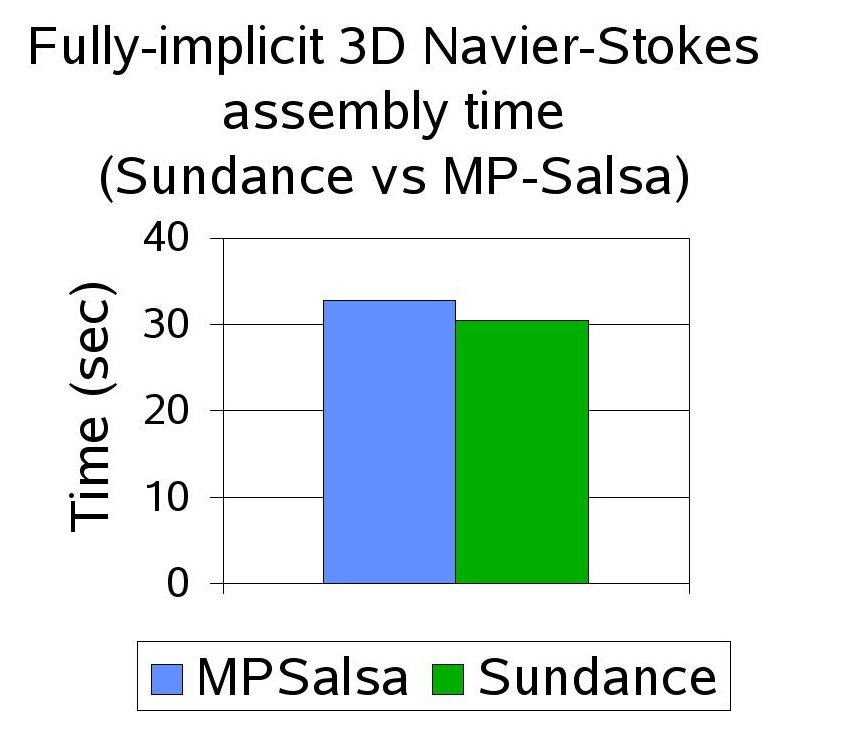
\epsfig{file=mpsalsa-timings.jpg,height=2.4cm}
\end{figure}
\begin{figure}
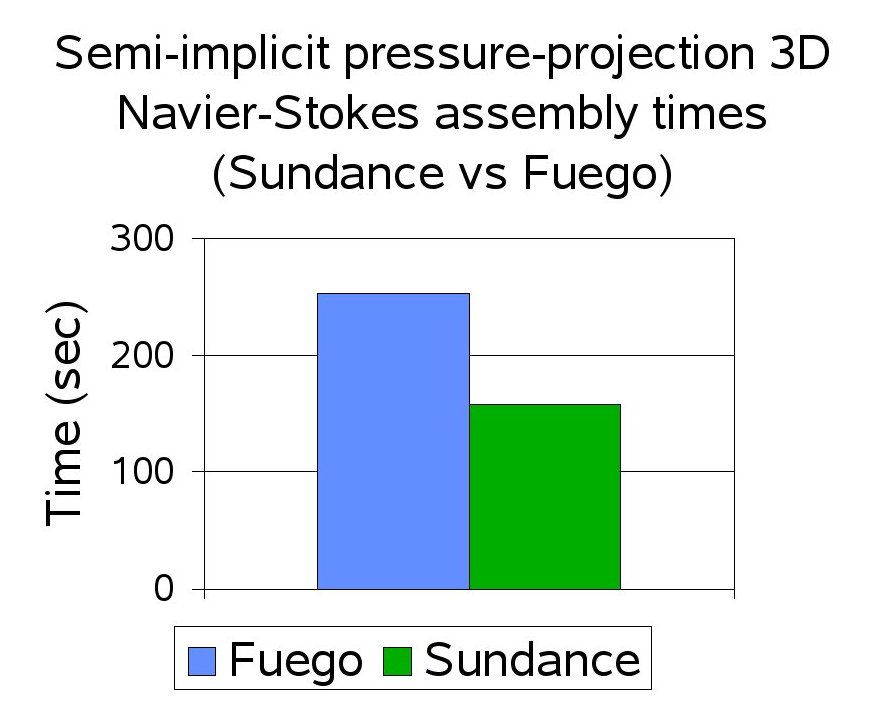
\epsfig{file=fuego-timings.jpg,height=2.4cm}
\end{figure}
\end{column}
\end{columns}
}

\frame
{
  \frametitle{Comparison to generated code (Dolfin)}

  \begin{block}{}

\begin{center}
\begin{tabular}{|r|r||r|r|}
\hline
\multicolumn{4}{|c|}{Stokes assembly timings, 3D Taylor-Hood}\\
\hline
verts & tets    &  \multicolumn{2}{|c|}{$p=2;1$} \\
\hline
      &  &  Sundance & Dolfin\\
\hline
  &      &            &        \\
  142 & 495 & 0.07216 & 0.3362 \\
 874 & 3960 & 0.6677 & 2.793 \\
 6091 & 31680 & 5.521 & 22.57 \\
 45397 & 253440 & 45.97 & crash\\
\hline
\end{tabular}
\end{center}
  \end{block}

}

\frame
{
  \frametitle{Parallel scalability of assembly process}

  \begin{block}{}
  \begin{center}
  \begin{tabular}{|r|r|} \hline
  Processors & Assembly time \\ \hline
  4   &  54.5 \\ \hline
  16  &  54.7 \\ \hline
  32  &  54.3   \\ \hline
  128 &  54.4   \\ \hline
  256 &  54.4  \\ \hline
  \end{tabular}
  \end{center}
  \begin{itemize}
  \item Assembly times for a model CDR problem on ASC Red Storm
  \item Weak scalability means: assembly time remains constant as number of
processors increases in proportion to problem size
  \item Results demonstrate Sundance is weakly scalable
  \end{itemize}
  \end{block}

}


\frame
{
  \frametitle{How can user-friendly, intrusion-friendly code be fast?}

  \begin{block}{High performance is a result of:}
  \begin{itemize}
  \item Amortization of overhead
  \item Careful memory management
  \item Effective use of BLAS
  \item Work reduction through data flow analysis
  \end{itemize}
 \begin{center}
\textcolor{blue}
 {With our unified formulation, effort spent tuning computational kernels applies
immediately to diverse problem types and arbitrary PDE}
 \end{center}
  \end{block}

}


\frame
{
  \frametitle{A key to high level ease-of-use
without low performance: division of labor}

  \begin{alertblock}{Decouple {\bf user-level representiation}
from {\bf low-level evaluation}}
  \end{alertblock}

  \begin{block}{Reduces human factors / performance tradeoffs}
  \begin{itemize}
  \item User-level objects optimized for human factors
  \item Low-level objects optimized for performance
  \end{itemize}
  \end{block}

  \begin{block}{Allows interchangeable evaluators under a common interface}
  \begin{itemize}
  \item Easy to upgrade, tune, and experiment with evaluators w/o impact on user
  \item Future: different evaluators for different architectures
  \end{itemize}
  \end{block}
}



\end{document}
